\section{Nanoribbons}
\label{sec:nanoribbon}

In this section, we apply our code to the case of the honeycomb lattice of graphene and of the triangular lattice with nonuniform hoppings considered in the 3-band minimal model of \acs{TMD}s.
We take boundary conditions corresponding to nanoribbons.
These structures are much longer on one direction than on the other, , i.e. $l \gg w$, resembling a ribbon, hence their name.
This condition corresponds to taking $N_x \gg N_y$ in our conventions (see Fig.(\ref{fig:nanoribbon})\footnote{In Fig.(\ref{fig:nanoribbon}, this condition is, of course, not obeyed solely for the sake of giving a good visual representation of the boundary conditions, and the numbering system).}.
The low energy electronic states on the edges of these ribbons might lead to nontrivial magnetic behavior in \ac{TMD} nanostructures (as indeed they do in graphene nanostructures \cite{yazyev_emergence_2010}) and it is this possibility was unexplored numerically before this work \cite{feldner_dynamical_2011, golor_quantum_2013}, as was mentioned on chapter \ref{cap:int}.

\subsection{Graphene}
\label{sec:graphene}

We use three coordinates to label each site on the honeycomb lattice, by taking advantage of its bipartite nature.
Regarding the honeycomb lattice as two interpenetrating triangular sublattices $\mathcal{A}$ and $\mathcal{B}$, we take the axes $x$ and $y$ to be along the primitive vectors of each triangular sublattice.
Along the $x$-direction, a ribbon is normally very long, which justifies the fact that we take \acp{PBC}.
In contrast, in the narrow $y$-direction we take \acp{OBC}.
To number the sites on the ribbon, we introduce an additional coordinate labeling the sublattice: $z = 0$, if the site is in sublattice $\mathcal{A}$, and $z = 1$ if the site is in sublattice $\mathcal{B}$.
We then adopt the numbering convention for the sites $i = 0,1, ..., 2 N_x N_y - 1$ of the lattice $\mathcal{L}$:
$
i (x, y, z) = N_x N_y z + N_x y + x,
$
 where $x = 0, ..., N_x - 1$, $y = 0, ..., N_y - 1$, and $z = 0, 1$ define each element $\bm r = (x, y, z) \in \mathcal{L}$.

\begin{figure}[H]\label{fig:bcRibbon}
	\centering
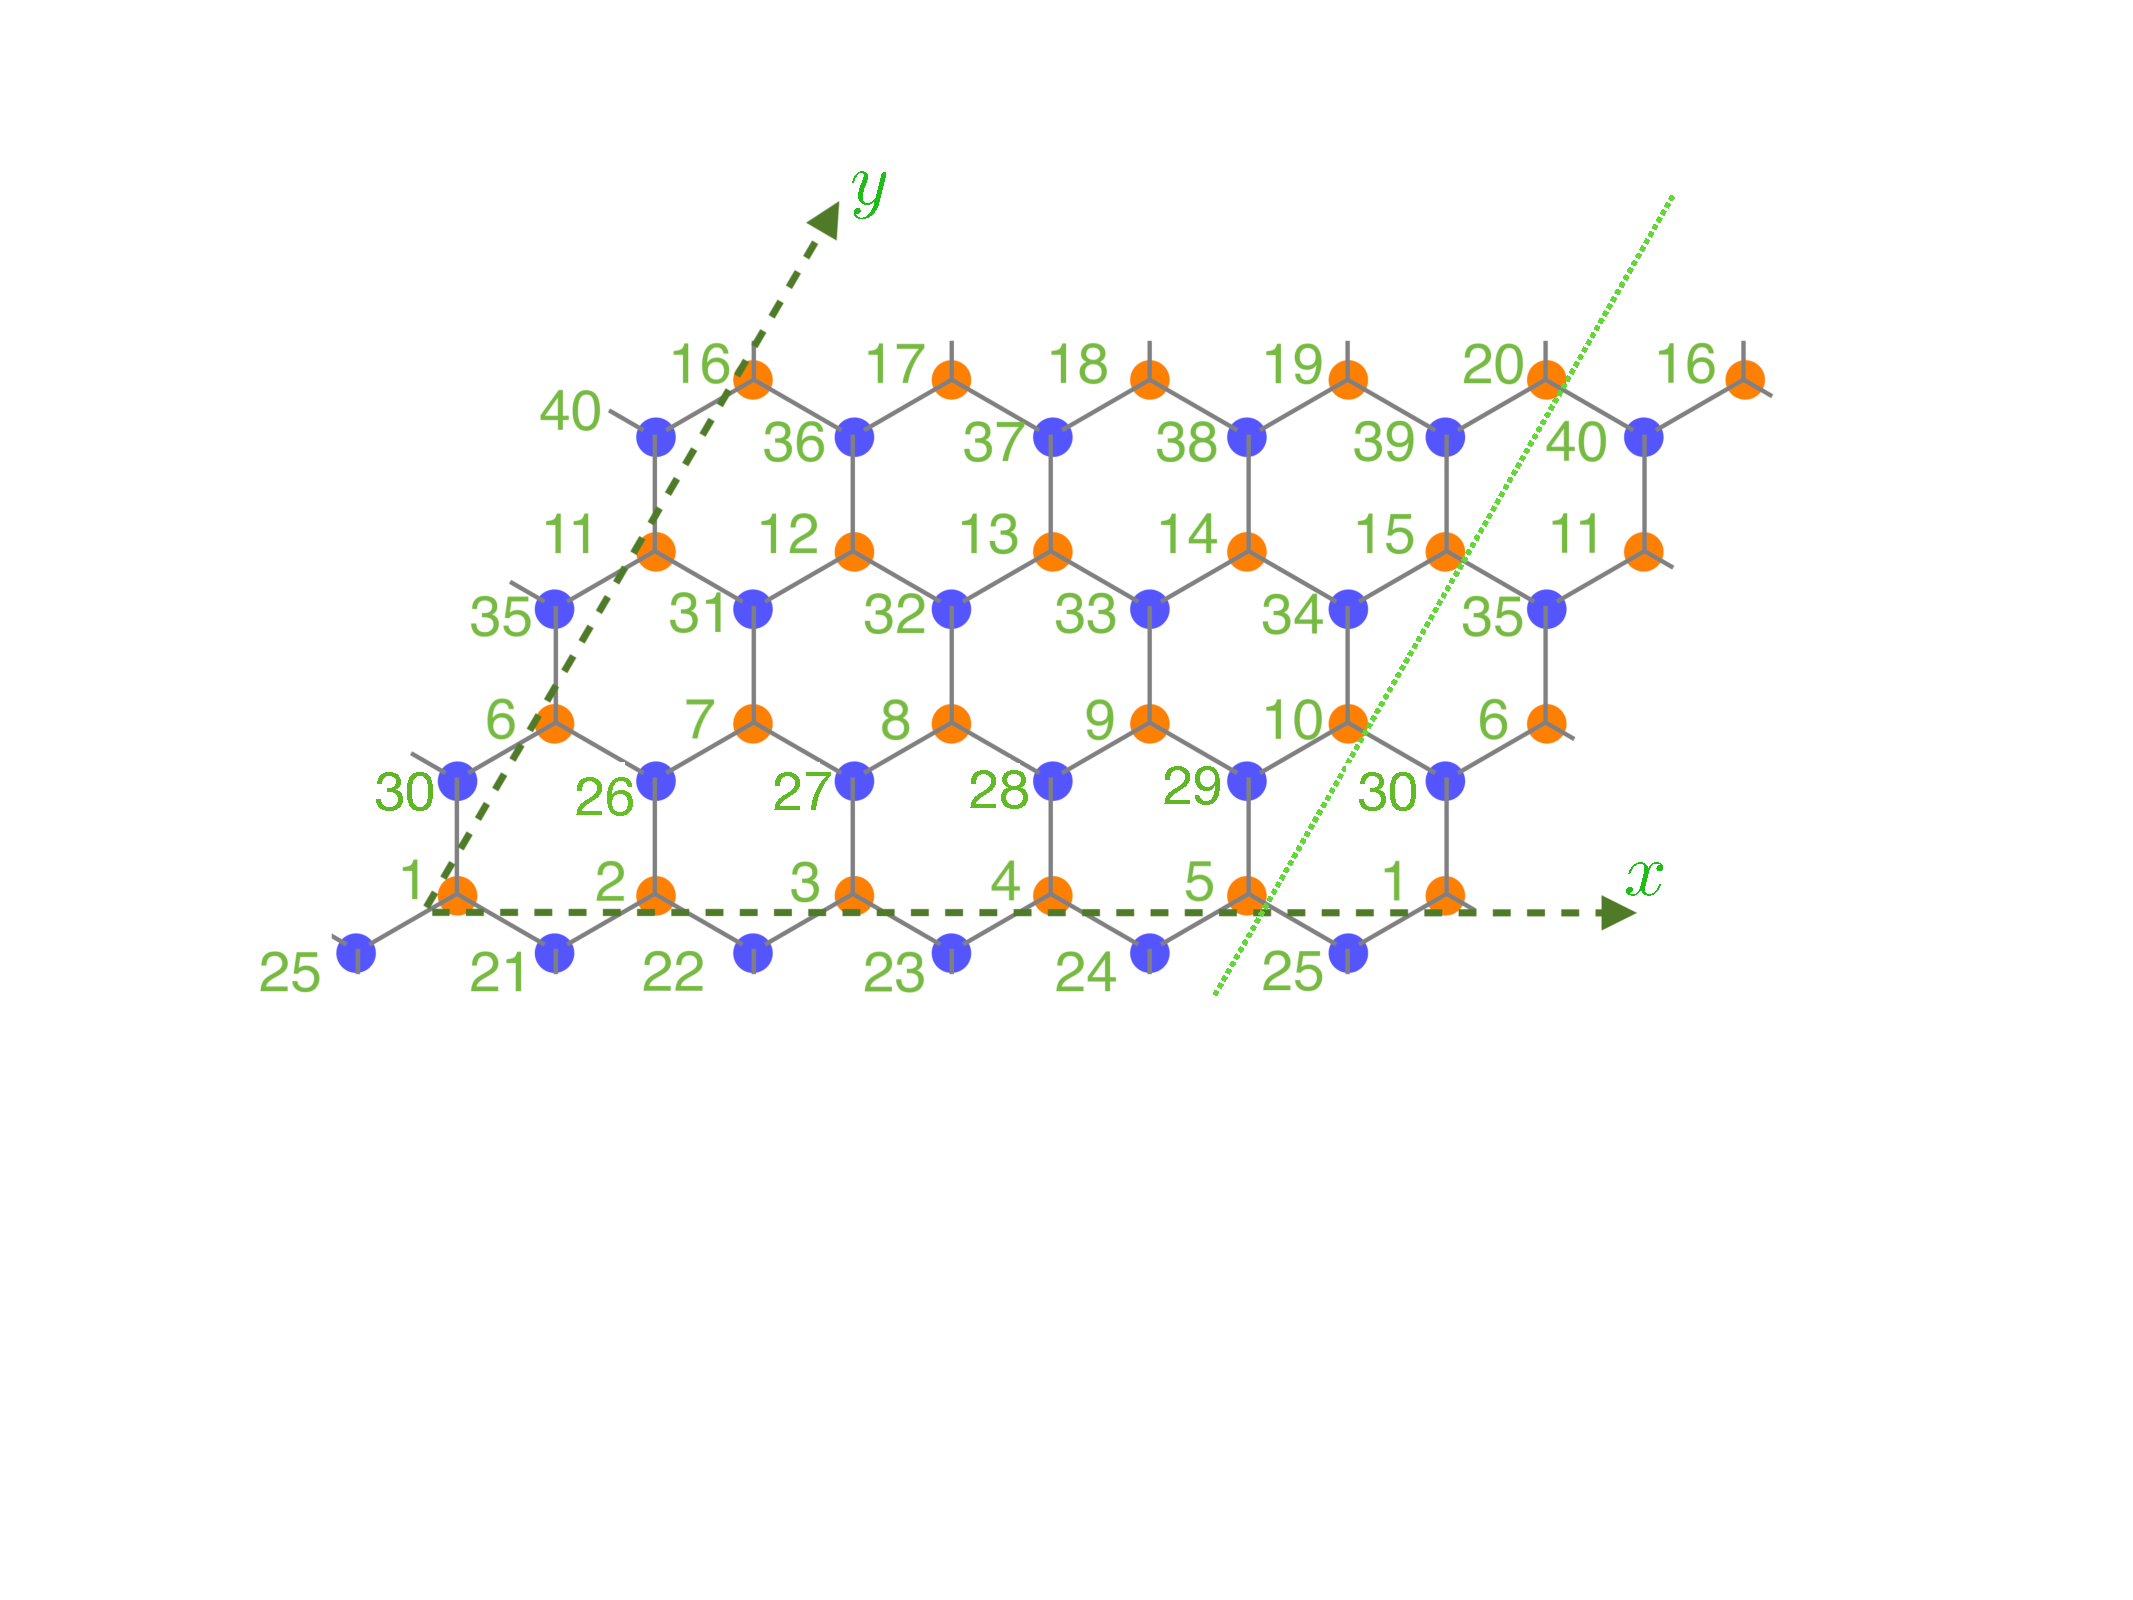
\includegraphics[trim={0 8cm 0 2.5cm},clip, scale = 0.25]{Applications/nanoribbon.pdf}
	\caption[Boundary conditions on the nanoribbon.]{Boundary conditions on the nanoribbon for $N_x = 5, \, N_y = 4$. The orange circles correspond to sublattice $\mathcal{A}$, and the blue circles correspond to sublattice $\mathcal{B}$.
	The counting starts at 1 (i.e. the numbers correspond to $i+1$, since $i$ starts at 0).}
	\label{fig:nanoribbon}
\end{figure}

The geometry of the system appears through the hopping matrix $\bm K$ in our code.
This numbering system makes it straightforward to find the neighbors of each site.
Let us begin by considering a site that is not on a zigzag edge.
There are two possible cases. For example, for 
$
z_i = 0, y_i \neq N_y - 1, x_i \neq 0 ,
$
 we have that the nearest neighbors of $i$ are $ j (i) = \{ j ( \bm r) \}$, with $\bm r$ in
\begin{equation*}
\bigg\{ \bm r_j \in \mathcal{L} \bigg| z_j = 1 \,\land\, \bigg[ \bigg( y_j = y_i  \,\land\, ( x_j = x_i \,\lor\, x_j = x_i - 1) \bigg) \,\lor\, \bigg( y_j = y_i + 1  \,\land\, x_j = x_i - 1  \bigg)  \bigg] \bigg\}
\end{equation*}

As opposed to the sites of a honeycomb lattice with \acp{PBC}, which have 3 neighbors, the sites of the zigzag edges have only 2 neighbors.
We summarize all possible cases in the following table.

\begin{table}[H]
\centering
	\caption{Nearest neighbors on the graphene nanoribbon.
	The neighbors in gray are only for sites that are not on the edges.
	$\%$ refers to the remainder of integer division.}
	\begin{tabular}{|c|c|c|c|} \hline
	\multicolumn{4}{|c|}{\textbf{\acp{OBC} \color{silver}{(\acp{PBC})} }}							\\ \hline
		Case 				& $z_j$	& $y_j$	& $x_j$ 	\\ \hline
		\multicolumn{1}{|c|}{\multirow{3}{*}{$z_i = 0$}}	 &	\multicolumn{1}{c|}{\multirow{3}{*}{1}} & \multicolumn{1}{c|}{\multirow{2}{*}{$y_i$}} & $x_i$   \\ \cline{4-4}
	   	\multicolumn{1}{|c|}{}	& \multicolumn{1}{c|}{\multirow{3}{*}{}} & \multicolumn{1}{c|}{\multirow{2}{*}{}}& \multicolumn{1}{c|}{\multirow{2}{*}{$N_x - 1 - (N_x - x_i) \% N_x$}} \\ \cline{3-3}
	   	\multicolumn{1}{|c|}{}	& \multicolumn{1}{c|}{} & \color{silver}{$y_i +1$} & \multicolumn{1}{c|}{\multirow{2}{*}{}} \\ \hline
		\multicolumn{1}{|c|}{\multirow{3}{*}{$z_i = 1$}}	 &	\multicolumn{1}{c|}{\multirow{3}{*}{0}} & \multicolumn{1}{c|}{\multirow{2}{*}{$y_i$}} & $x_i$   \\ \cline{4-4}
	   	\multicolumn{1}{|c|}{}	& \multicolumn{1}{c|}{\multirow{3}{*}{}} & \multicolumn{1}{c|}{\multirow{2}{*}{}}& \multicolumn{1}{c|}{\multirow{2}{*}{$(x_i + 1) \% N_x$}} \\ \cline{3-3}
	   	\multicolumn{1}{|c|}{}	& \multicolumn{1}{c|}{} & \color{silver}{$y_i -1$} & \multicolumn{1}{c|}{\multirow{2}{*}{}} \\ \hline
	\end{tabular}
	\label{tab:dummytable}
\end{table}

\subsection{\acp{TMD}}
\label{subsec:apTMD}

We start by approaching the \acs{TMDNR} problem at the mean field level.
Such a procedure is very useful to obtain a physical picture of the system's behavior.
In particular, at a given temperature, if there is a transition between a configuration with magnetic order, and a disordered one, there is a critical interaction parameter $U = U_c$ at which the transition occurs, and it can be estimated in mean field, and compared with the more precise, unbiased \acs{QMC} result.
In general, our mean field formulation would involve diagonalizing an $N \times N$ matrix at each step, where $N = N_{\text{orb}} N_x N_y$ is the size of the system times the number of orbitals.
However, since we consider \acs{PBC}s along the $x$-direction, we can partially diagonalize  the Hamiltonian analytically, reducing the size of the matrix to be diagonalized to $N_{\text{orb}} N_y \times N_{\text{orb}} N_y$, where $N_y$ is the width of the ribbon, i.e. the number of $\text{M}\text{X}_2$ formula units.
Consider the spinless 3-band tight binding model, with the lattice constant: $a \equiv 1$.
\begin{equation}
\begin{split}
\mathcal{H}_0 &= \sum_{\substack{m, n \\ \alpha, \beta}} \bigg( c_{m,n, \alpha}^\dagger t_{\alpha\beta}^0 c_{m, n, \beta} + \delta_{0, N_x}  c_{m,n, \alpha}^\dagger t_{\alpha\beta}^1 c_{m+1, n, \beta} + \delta_{-\sqrt{3}/2, (N_y -1)\sqrt{3}/2}  c_{m,n, \alpha}^\dagger t_{\alpha\beta}^4 c_{m-1, n, \beta} \\
& + \delta_{0, N_m} \delta_{-1, (N_y -1)\sqrt{3}/2} c_{m+1/2,n-\sqrt{3}/2, \alpha}^\dagger t_{\alpha\beta}^2 c_{m, n, \beta} + \delta_{-1, (N_y -1)\sqrt{3}/2} c_{m-1/2,n-\sqrt{3}/2, \alpha}^\dagger t_{\alpha\beta}^3 c_{m, n, \beta} \\
& + \delta_{N_y\sqrt{3}/2, 0} c_{m+1/2,n+\sqrt{3}/2, \alpha}^\dagger t_{\alpha\beta}^6 c_{m, n, \beta} + \delta_{-1, N_x -1} \delta_{N_y\sqrt{3}/2, 0} c_{m-1/2,n+\sqrt{3}/2, \alpha}^\dagger t_{\alpha\beta}^5 c_{m, n, \beta} \bigg)
\end{split}
\end{equation}

Fourier transforming along $m$: $c_{m, n, \alpha} = \frac{1}{\sqrt{N_x}}\sum_{k} e^{-i k m } c_{k, n, \alpha} $, with $k = \frac{2\pi}{N_x} \{ -\frac{N_x}{2} + 1, -\frac{N_x}{2}, ..., \frac{N_x}{2} \}$:
\begin{equation}
\begin{split}
\mathcal{H}_0 &= \sum_{ \substack{k, y \\ \alpha, \beta} } \bigg( c_{k, y, \alpha}^\dagger (t_{\alpha \beta}^0  + e^{ik} t_{\alpha \beta}^1 + e^{-ik} t_{\alpha \beta}^4 )  c_{k, y, \beta} + \delta_{-1, N_y -1} c_{k, y - 1, \alpha}^\dagger ( e^{ik/2} t_{\alpha \beta}^2 + e^{-ik/2} t_{\alpha \beta}^3 ) c_{k, y, \beta} \\
& + \delta_{N_y, 0} c_{k, y, \alpha}^\dagger ( e^{ik/2} t_{\alpha \beta}^6 + e^{-ik/2} t_{\alpha \beta}^5 ) c_{k, y+1, \beta} \bigg) , \,\, \text{with} \, y \, \text{defined as in Fig.(4.1)}
\end{split}
\end{equation}
leading to a tridiagonal block $3 N_y \times 3 N_y$ hopping matrix $\bm H (k)$ with three different types of matrix elements: $\bm h_1 = \bm H_{y,y}$, $\bm h_2 = \bm H_{y,y-1}$, $\bm h_2^\dagger = \bm H_{y, y+1}$.
\begin{equation}
[ H_{(\alpha y) (\beta y')} (k) ] = 
\begin{pmatrix}
\bm h_1 & \bm h_2^\dagger & & & \\
\bm h_2 & \bm h_1 & \bm h_2^\dagger & & \\
& \bm h_2 & \bm h_1 & \ddots & \\
& & \ddots & \ddots & \bm h_2^\dagger \\
& & & \bm h_2 & \bm h_1
\end{pmatrix}, \, 
\bm h_1 = 
\begin{pmatrix}
\varepsilon_1 + 2 t_0 \cos k & 2 i t_1 \sin k & 2 t_2 \cos k \\
-2 i t_1 \sin k & \varepsilon_2 + 2 t_{11} \cos k & 2 i t_{12} \sin k \\
2 t_2 \cos k& -2 i t_{12} \sin k & \varepsilon_2 + 2 t_{22} \cos k \\
\end{pmatrix}
\end{equation}
\begin{equation*}
\bm h_2 =
\begin{pmatrix}
2 t_0 \cos ( k / 2 ) & i \sin ( k / 2 ) \bigg( t_1 - \sqrt{3} t_2 \bigg) & - \cos (k /2 ) \bigg( \sqrt{3} t_1 + t_2 \bigg) \\
-i \sin ( k / 2 ) \bigg(t_1 + \sqrt{3} t_2 \bigg) & \frac{1}{2} \cos (k / 2) \bigg( t_{11} + 3 t_{22} \bigg) & -i \sin (k / 2) \bigg( \frac{\sqrt{3}}{2} (t_{11} -  t_{22} ) + 2 t_{12} \bigg) \\
\cos ( k / 2) \bigg( \sqrt{3} t_1 - t_2 \bigg) & -i \sin (k / 2) \bigg( \frac{\sqrt{3}}{2} ( t_{11} - t_{22} ) - 2 t_{12} \bigg) & \frac{1}{2} \cos (k / 2) \bigg( 3 t_{11	} + t_{22} \bigg)
\end{pmatrix}
\end{equation*}
\begin{figure}[H]
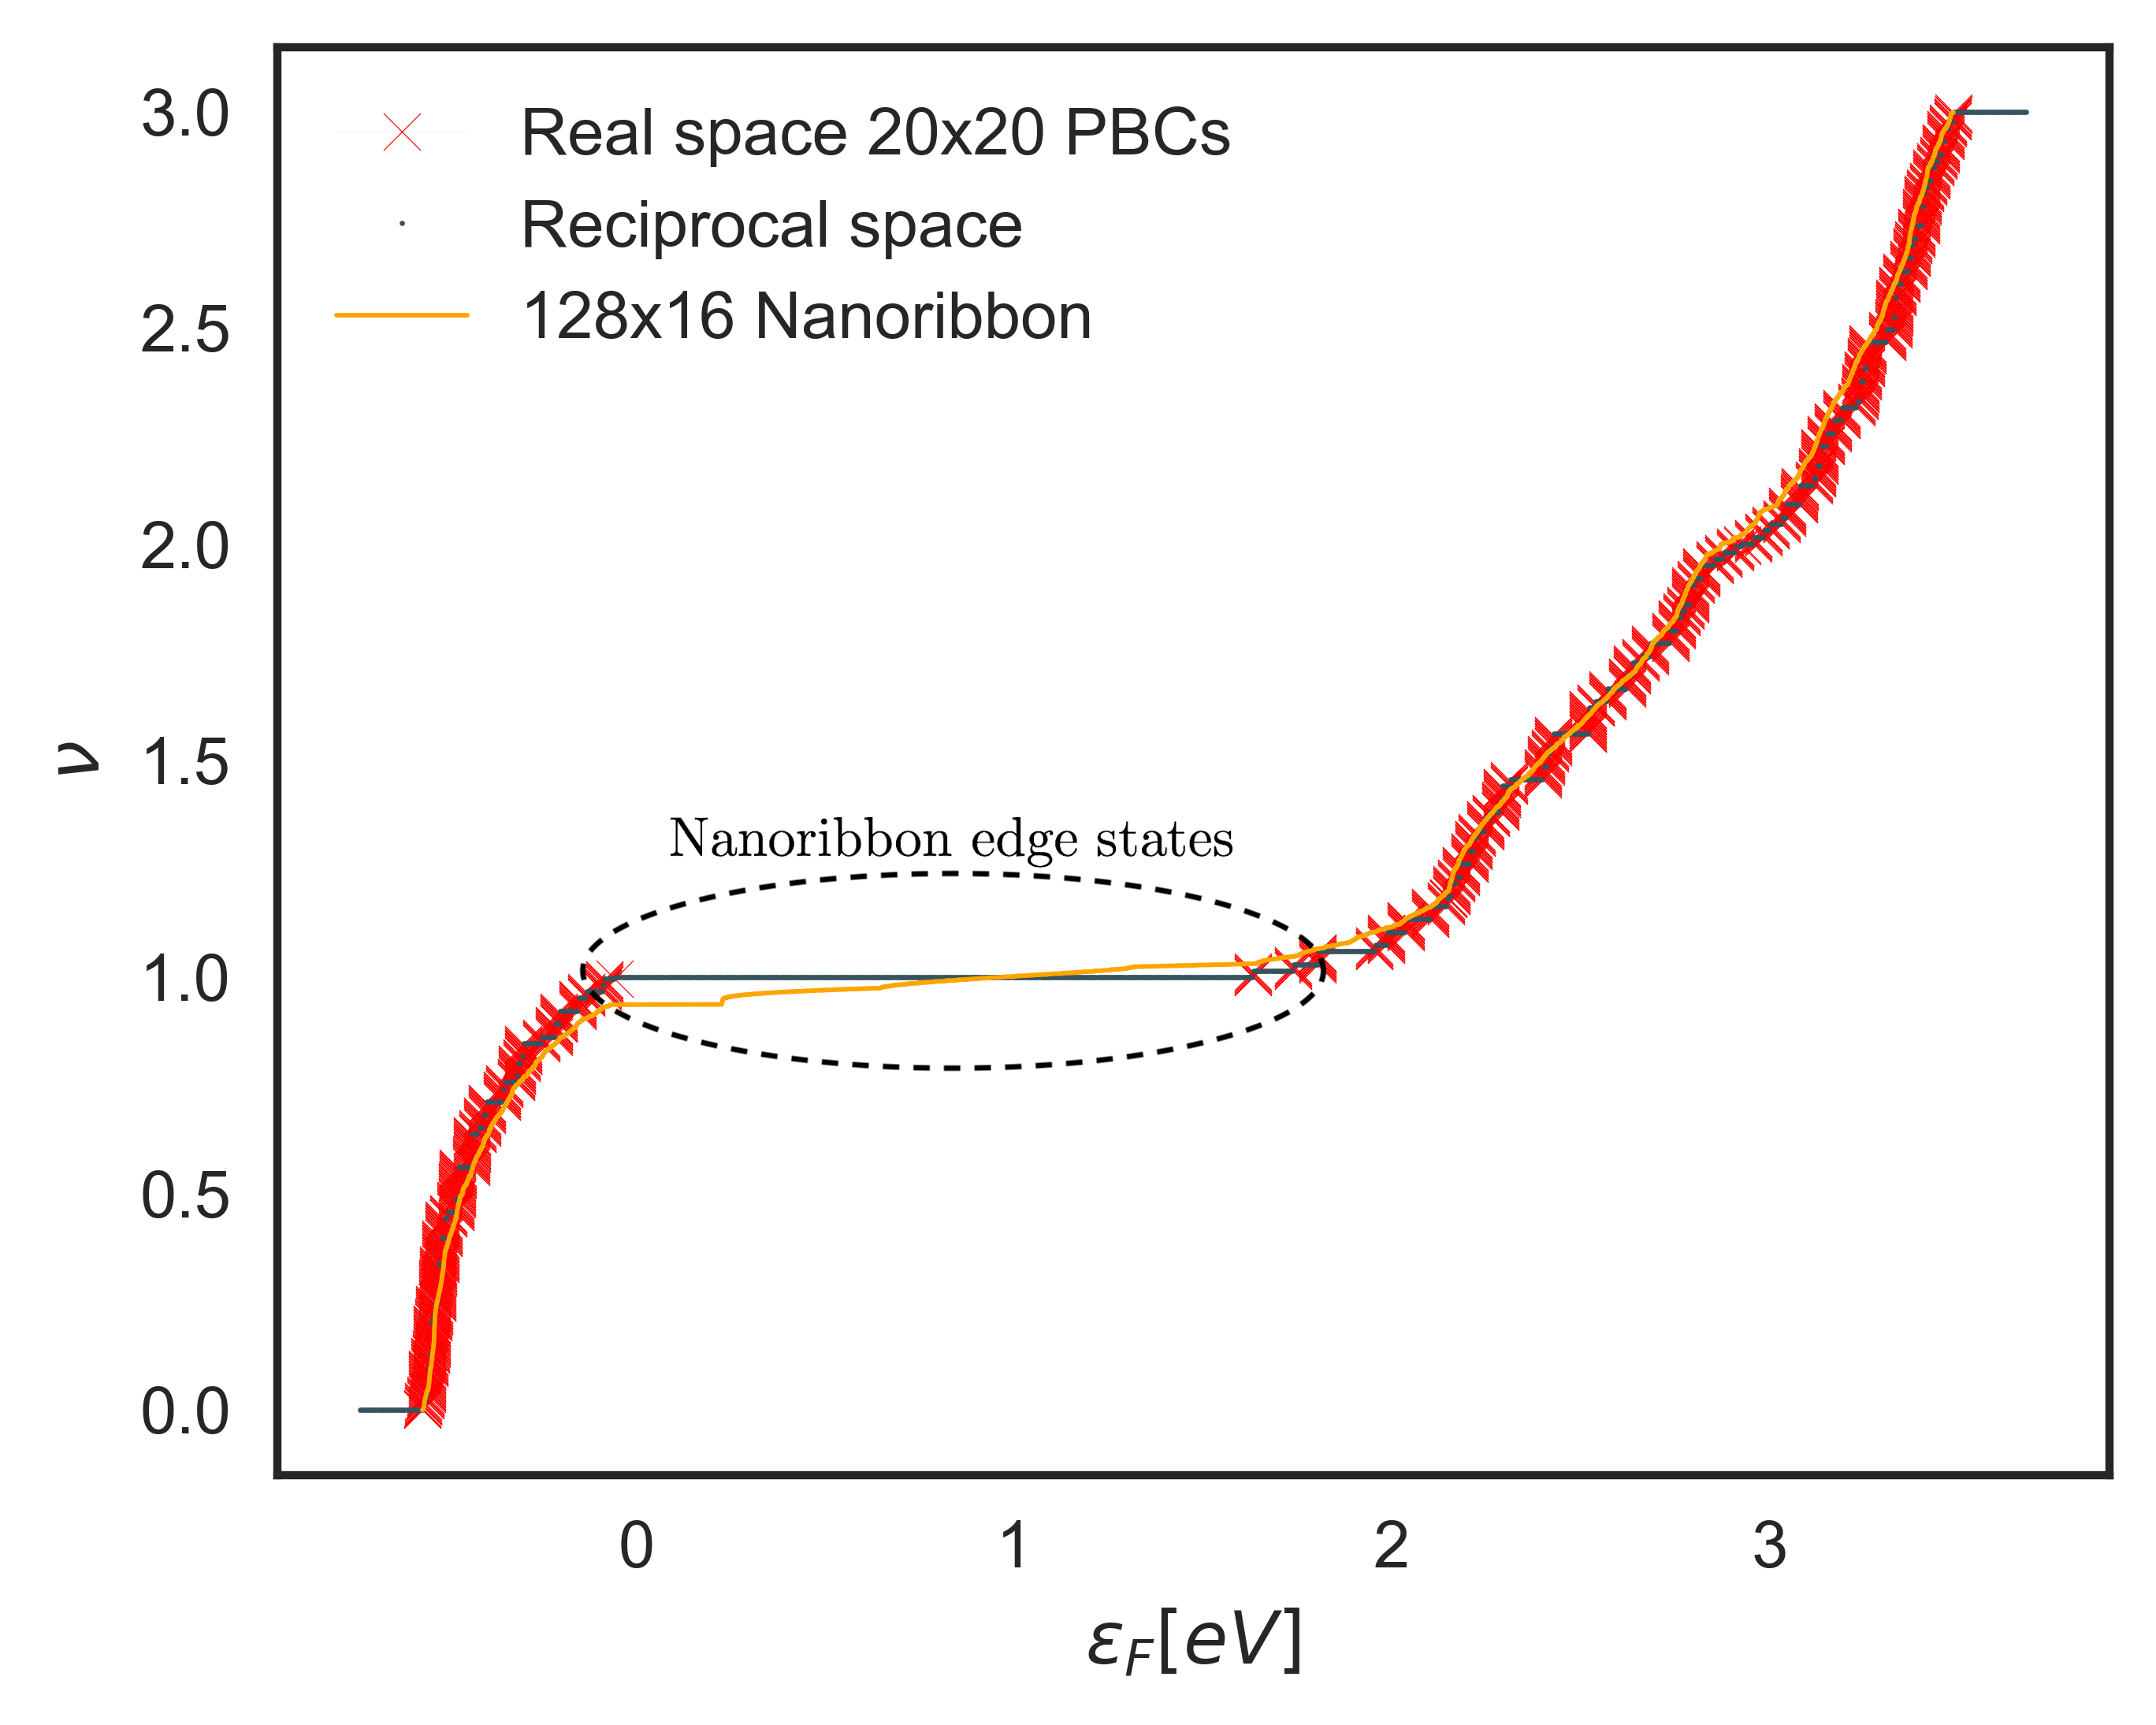
\includegraphics[scale=0.55]{Applications/fillingVsE.png}
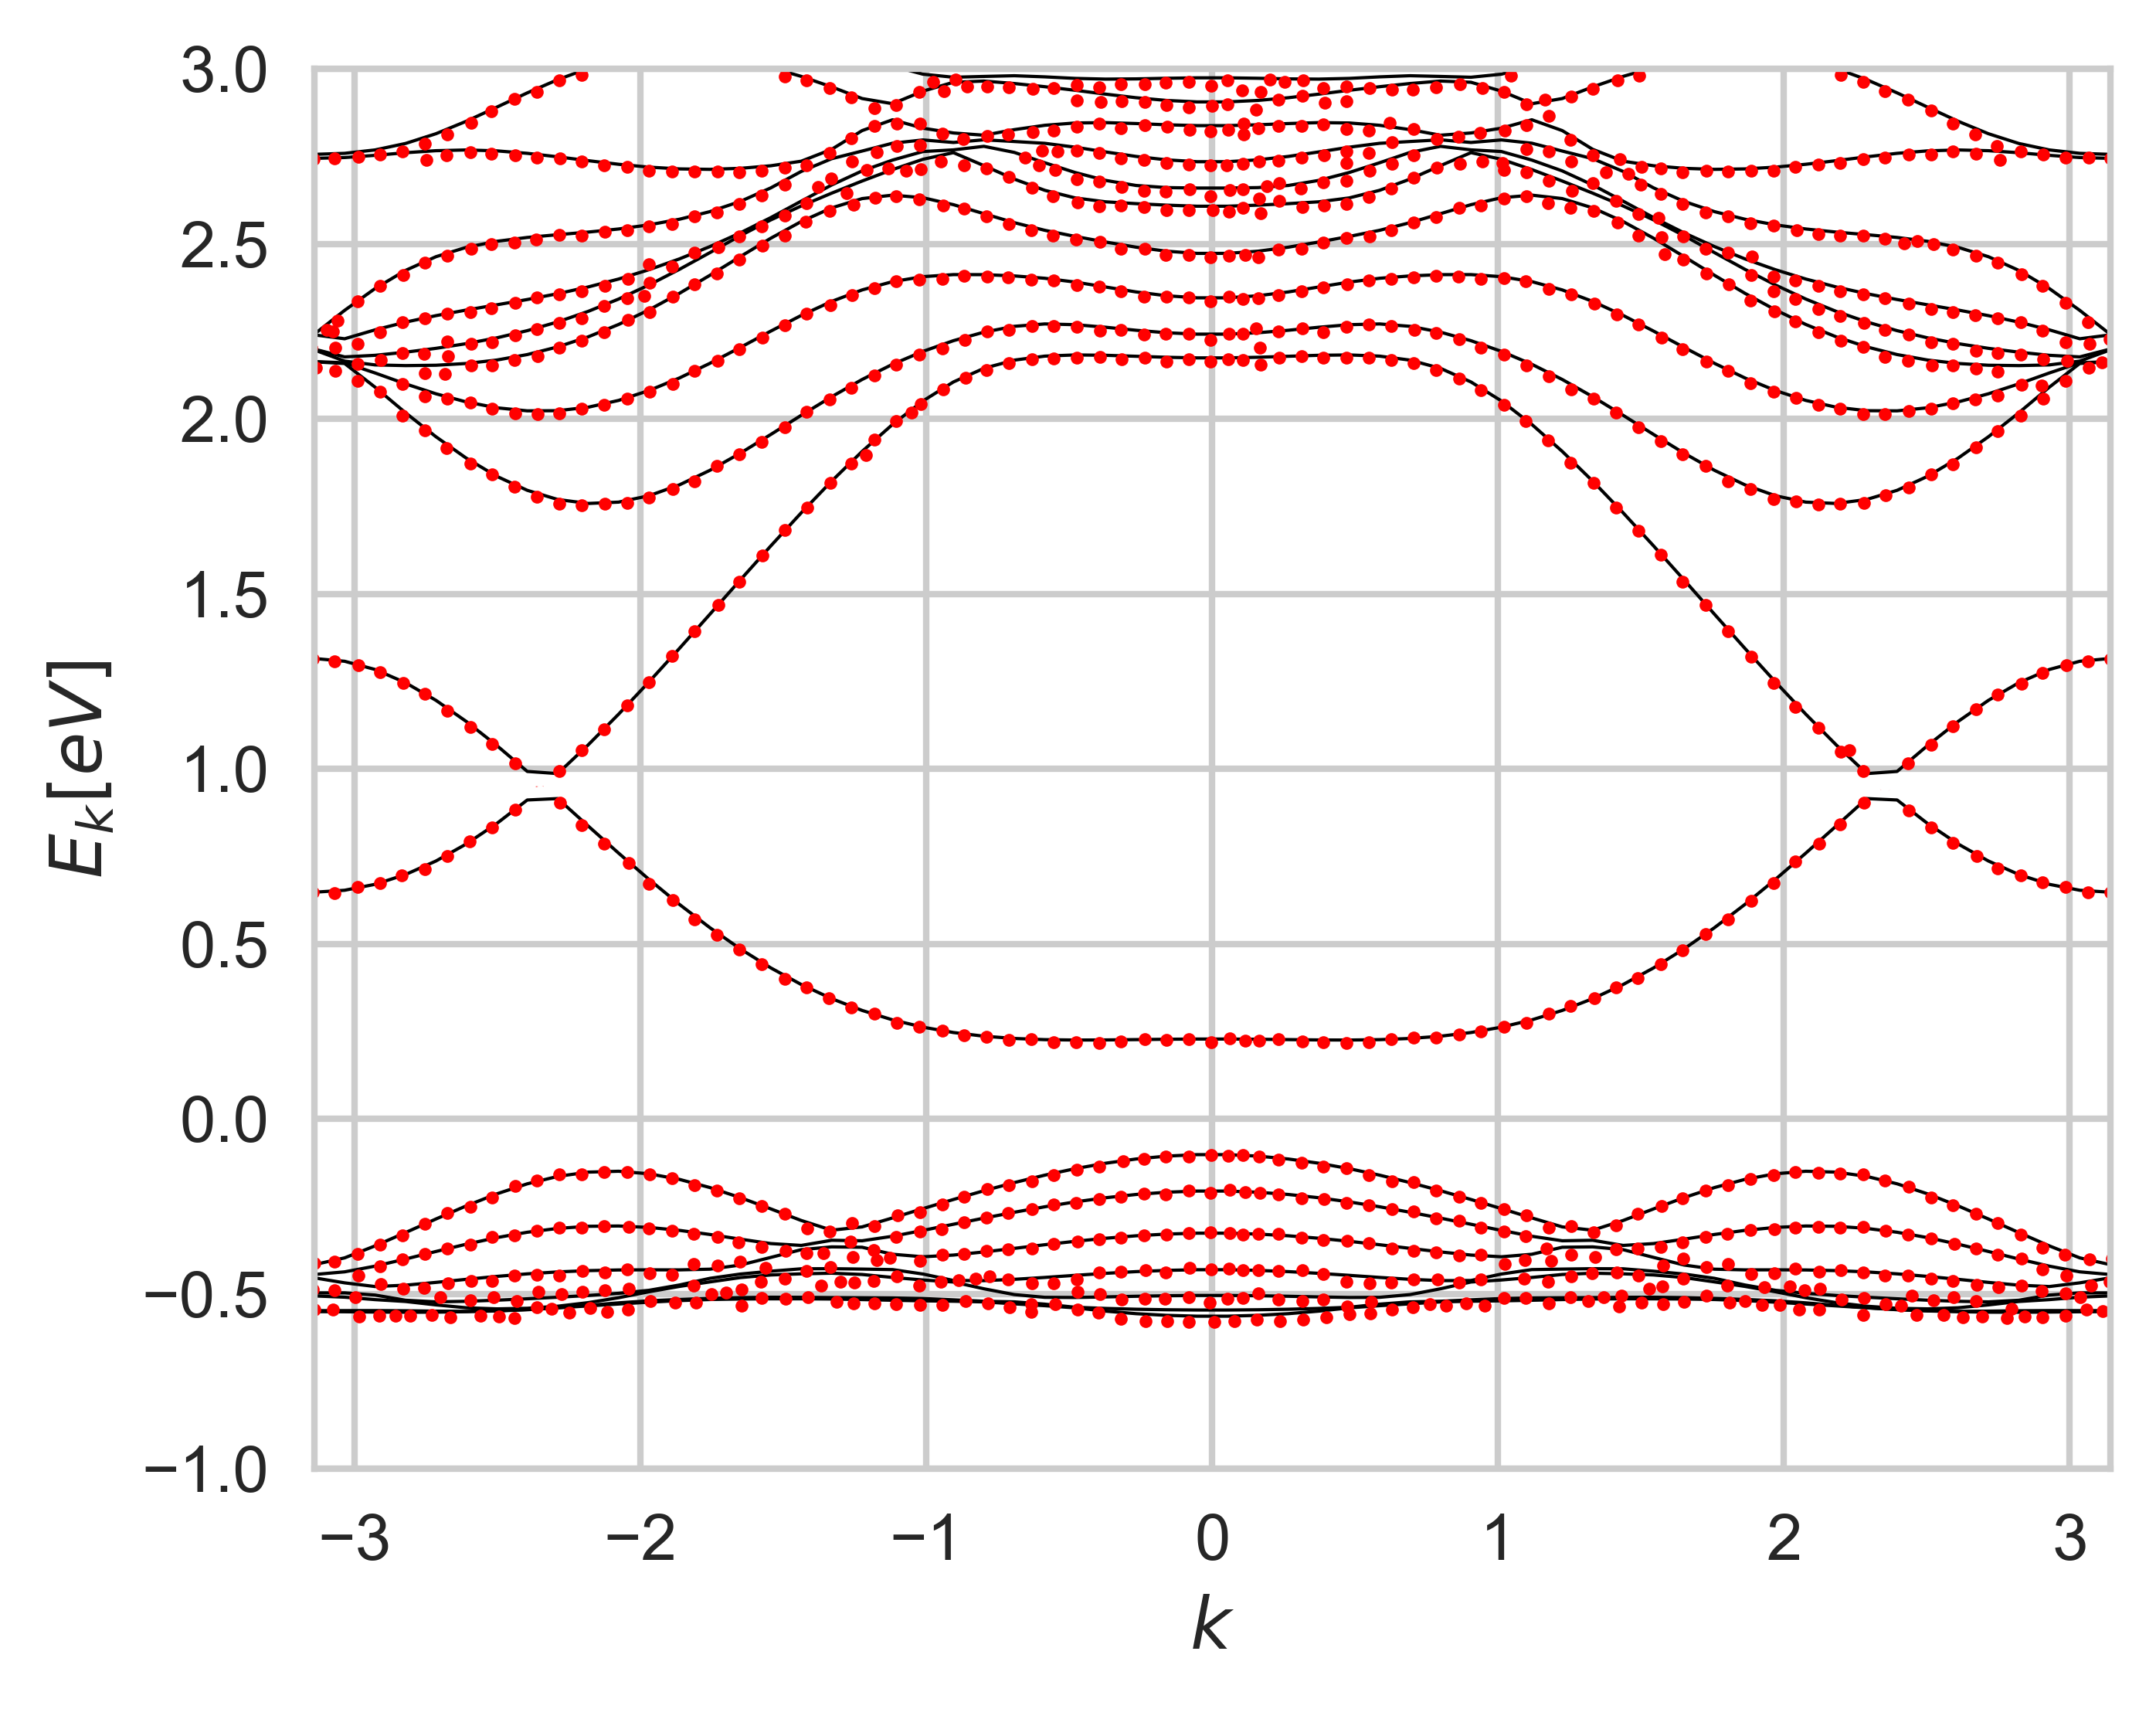
\includegraphics[scale=0.55]{Applications/BandStructureNanoribbonTMD.png}
	\caption[Filling $\nu$ as a function of the Fermi energy $\varepsilon_F$ for a \acs{TMD} monolayer and a nanoribbon. $\text{Mo}\text{S}_2$.  \acs{TMDNR} band structure obtained by the 3-band model.]{Left: Filling $\nu$ as a function of the Fermi energy $\varepsilon_F$ for a system with \acp{PBC}, as computed by diagonalizing the input matrix of our code, and by the hopping matrix in $\bm k$-space. Comparison between the fillings of a nanoribbon and a periodic system.
	For the nanoribbon, edge states appear on the gap of the periodic system.
	Right: 3-band model $\text{Mo}\text{S}_2$ zigzag edged nanoribbon energy bands (red dots and orange curve), for $N_y = 8$, using the GCA parameters. The first principles bands show the contribution from orbitals that are not considered in the 3-band model (blue:  $d_{z^2}$, $d_{xy}$, $d_{x^2-y^2}$, green: others). The 3-band model reproduces the bands that correspond to the orbitals taken into account reasonably (1 and 2 correspond to the edge states from the $d_{z^2}$, $d_{xy}$, $d_{x^2-y^2}$ orbitals of the $\text{Mo}$ atoms, while 3 and 4 correspond to the $d_{yz}$ orbital at the $\text{Mo}$-terminated edge, and $p_{y, z}$ orbitals from the $\text{S}$-terminated edge, and are not taken into account in the 3-band model).\cite{liu_three-band_2013}.}
	\label{fig:fillingVsE}
\end{figure}

By applying our mean field approach to solve the 3-band model with Hubbard-type interactions, we obtain solutions that are independent of $x$, which motivates us to reduce the number of MF parameters by choosing a translationally invariant ansatz.
This is equivalent to taking $\left\langle n_{x, y,\alpha, \sigma}\right\rangle = \left\langle n_{y,\alpha, \sigma}\right\rangle  \forall x$ ($6 N_y$ parameters).
By reducing the number of parameters, convergence is facilitated, which allows us to evaluate whether the solution of Fig.(\ref{fig:nanoGraphVsTMD}) is robust, i.e. whether it corresponds to a metastable or not.
The mean field form of the interaction term with the reduced number of parameters changes, implying that the self-consistent relation of Eq.(\ref{eq:selfConsistent}) from which the local densities are computed changes as well.
\begin{equation}
\mathcal{H}_{\text{MF}} = \mathcal{H}_0 + \mathcal{H}_1 + \mathcal{C} , \,\text{where} \,\, \mathcal{H}_1 = U \sum_{m, n, \alpha}  \sum_\sigma n_{\substack{m, \sigma \\ n, \alpha}} \big\langle n_{\substack{m, -\sigma \\ n, \alpha}} \big\rangle  , \,\, \mathcal{C} = -U  \sum_{m, n, \alpha} \big\langle n_{\substack{m, \uparrow \\ n, \alpha}} \big\rangle \big\langle n_{\substack{m, \downarrow \\ n, \alpha}} \big\rangle
\end{equation}
\begin{equation}
\begin{split}
\mathcal{H}_1 + \mathcal{C} &= \frac{U}{N_x^{\,2}} \sum_{\substack{n \alpha \\ k_1 k_2 \\ k_3 k_4}} \underbrace{\sum_m e^{i [ (k_1 + k_3) - (k_2 + k_4) ] m}}_{N_x \delta_{k_4, k_1 + k_3 - k_2}} \bigg( \sum_\sigma c_{\substack{k_1, \sigma \\ n, \alpha}}^\dagger c_{\substack{k_2, \sigma \\ n, \alpha}} \underbrace{\big\langle c_{\substack{k_3, -\sigma\\ n, \alpha}}^\dagger c_{\substack{k_4, -\sigma \\ n, \alpha}} \big\rangle}_{\delta_{k_3, k_4} \big\langle n_{\substack{k_3,-\sigma \\ n, \alpha}} \big\rangle} - \underbrace{\big\langle c_{\substack{k_1, \uparrow \\ n, \alpha}}^\dagger c_{\substack{k_2  \uparrow \\n, \alpha}} \big\rangle}_{\delta_{k_1, k_2} \big\langle n_{\substack{k_2,\uparrow \\ n, \alpha}} \big\rangle} \underbrace{\big\langle c_{\substack{k_3, \downarrow \\ n, \alpha}}^\dagger c_{\substack{k_4, \downarrow \\ n, \alpha}} \big\rangle}_{\delta_{k_3, k_4} \big\langle n_{\substack{k_3,\downarrow \\ n, \alpha}} \big\rangle}  \bigg) \\
&= \frac{U}{N_x} \sum_{\substack{n \alpha \\ k_2 k_3}} \bigg( \sum_\sigma n_{\substack{k_2, \sigma \\ n, \alpha}} \big\langle n_{\substack{k_3, -\sigma \\ n, \alpha}} \big\rangle - \big\langle n_{\substack{k_2, \uparrow \\ n, \alpha}} \big\rangle \big\langle n_{\substack{k_3, \downarrow \\ n, \alpha}} \big\rangle \bigg) \equiv
U \sum_{k, \mu} \bigg( \sum_\sigma n_{k,\mu, \sigma} \big\langle n_{\mu, -\sigma} \big\rangle - \big\langle n_{\mu, \uparrow} \big\rangle \big\langle n_{\mu, \downarrow} \big\rangle \bigg)
\end{split}
\end{equation}
where we collapsed the indexes $(n, \alpha)$ into a single index $\mu$.
The self consistent relation allowing us to compute the new MF parameters at each step emerges by diagonalizing $\mathcal{H}_1$ in the $\mu$-subspace:
\begin{equation}
\big\langle n_{\mu, \sigma} \big\rangle = \frac{1}{N_x}\sum_{q, \nu} | Q_{q \sigma \mu, \nu} |^2 \rho ( \varepsilon_{q \nu \sigma} ) , \, \text{where} \,\, d_{q, \sigma, \nu} = \sum_\nu Q_{q \sigma \mu, \nu}^\star c_{q ,\sigma, \mu} ,  \, \text{and} \,\, \mathcal{H}_{\text{MF}} = \sum_{q, \nu, \sigma} \varepsilon_{q, \nu, \sigma} d_{q, \nu, \sigma}^\dagger d_{q, \nu, \sigma} + \mathcal{C}
\end{equation}
\begin{figure}[H]
\hspace{0.1cm}
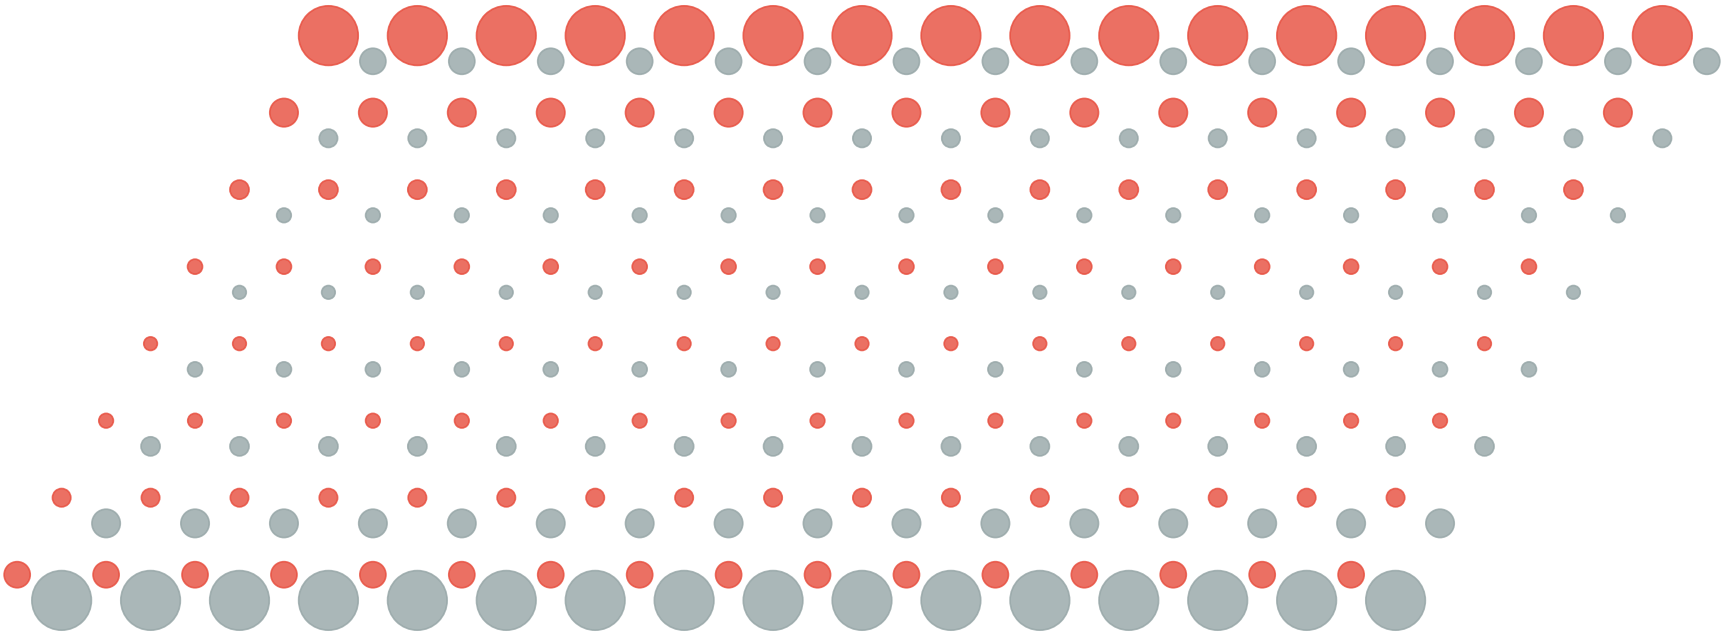
\includegraphics[scale=1.023]{Applications/MFnanoribbon.png}
\hspace{0.05cm}
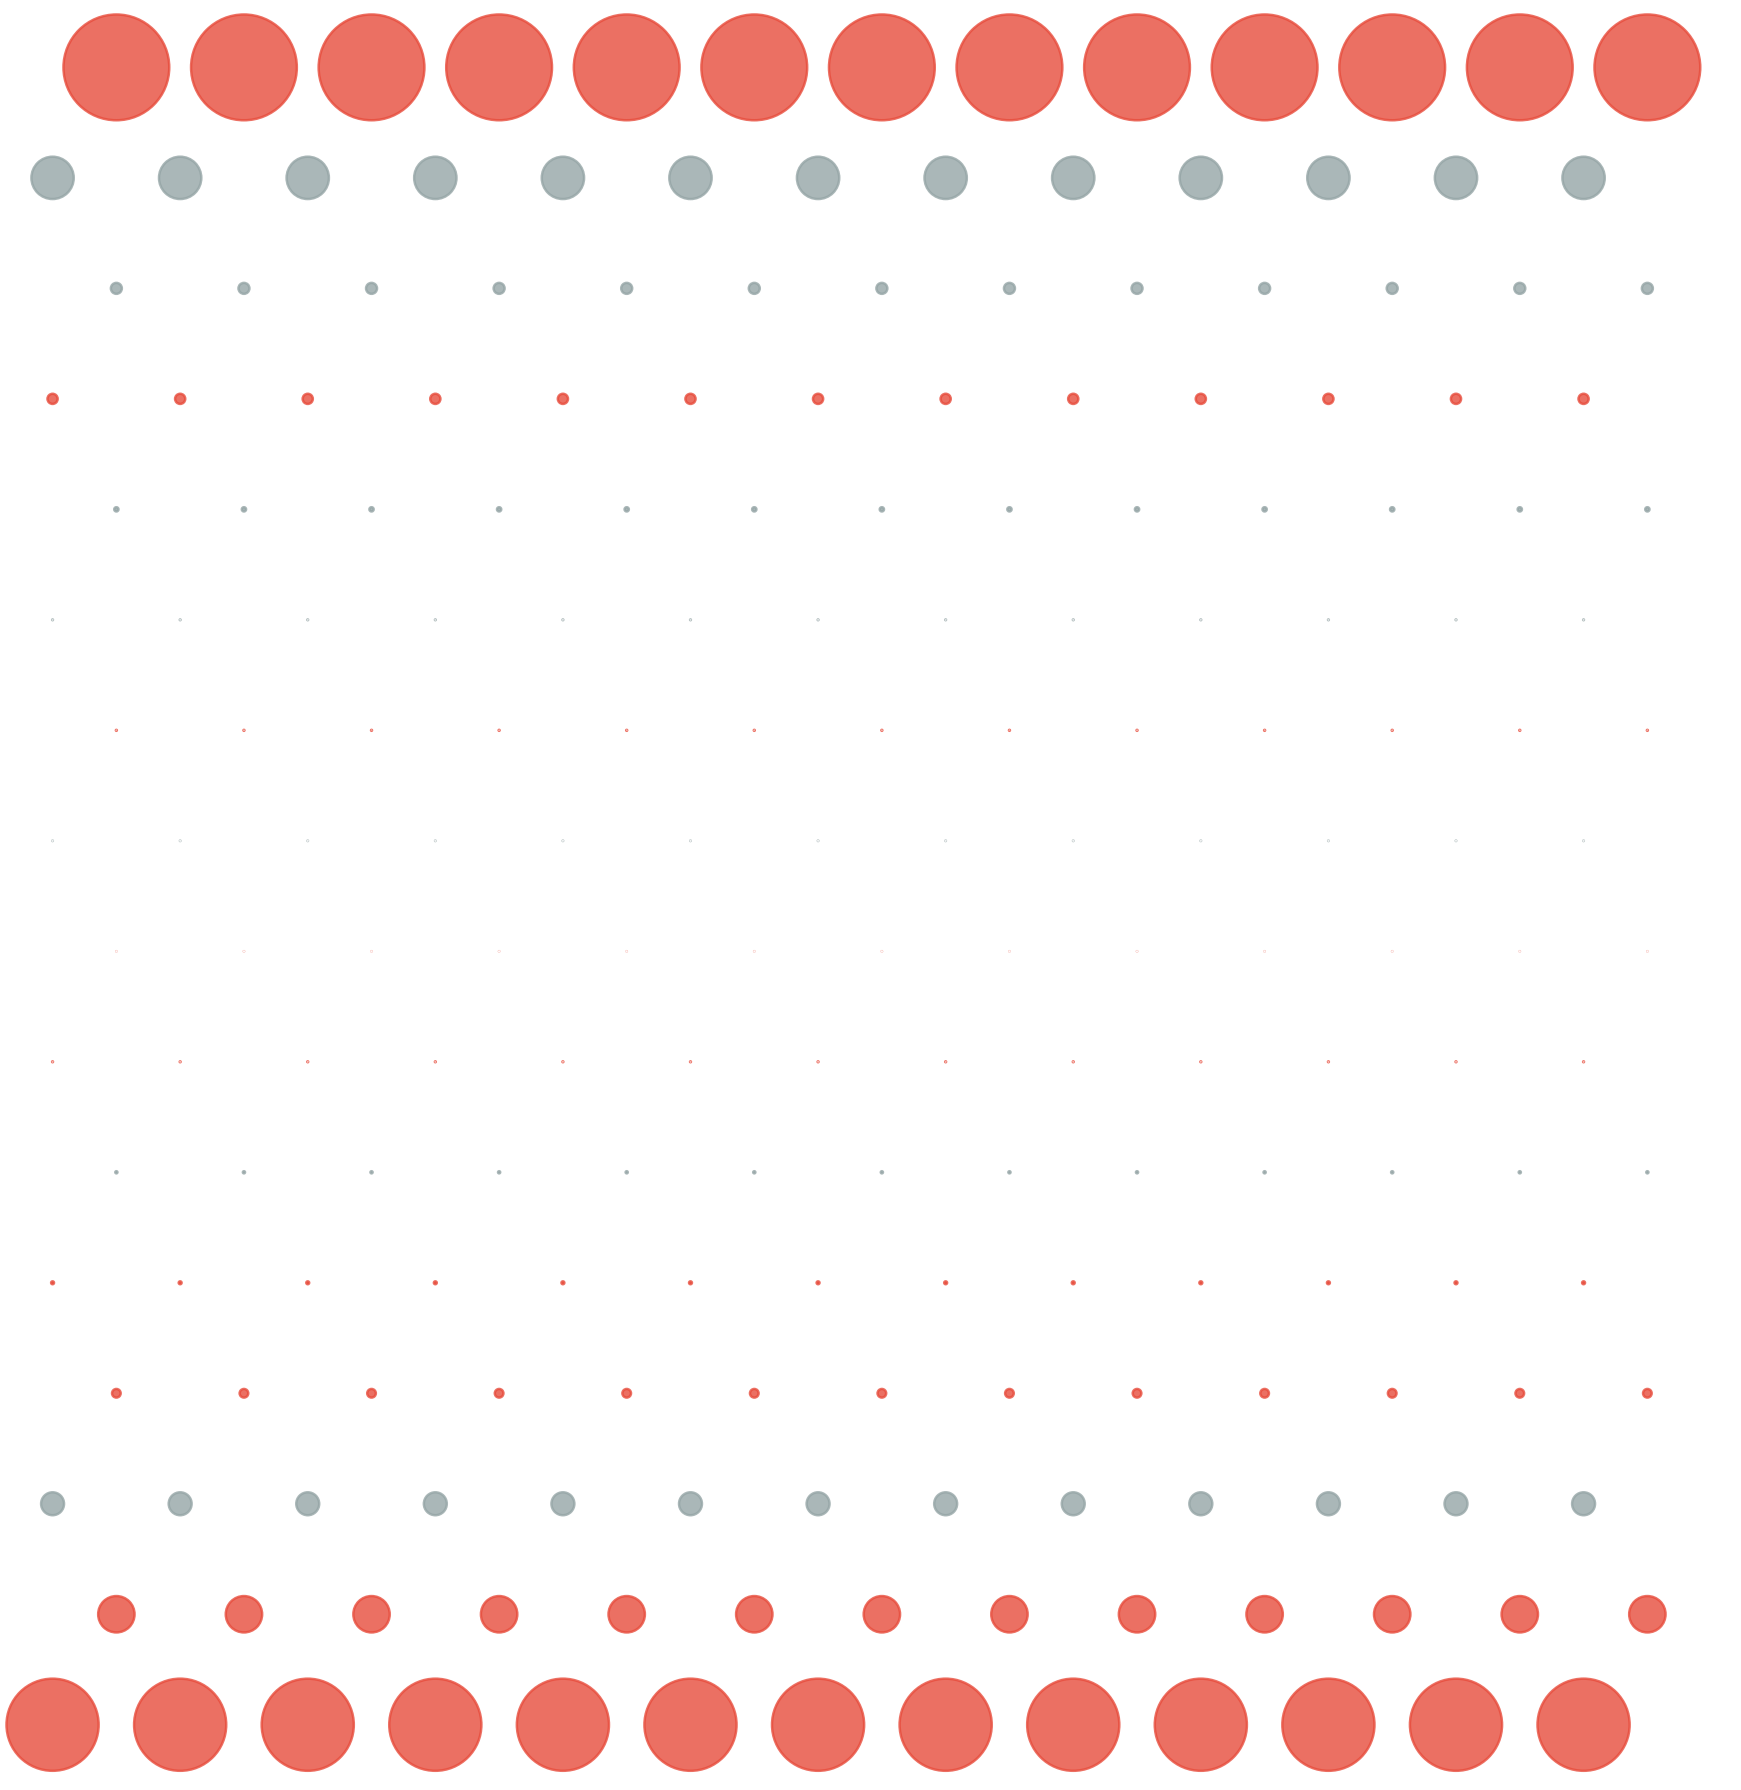
\includegraphics[scale=0.55]{Applications/lattice_Nx=512_Ny=16_U=20_beta=100.png}
\hspace{1cm}
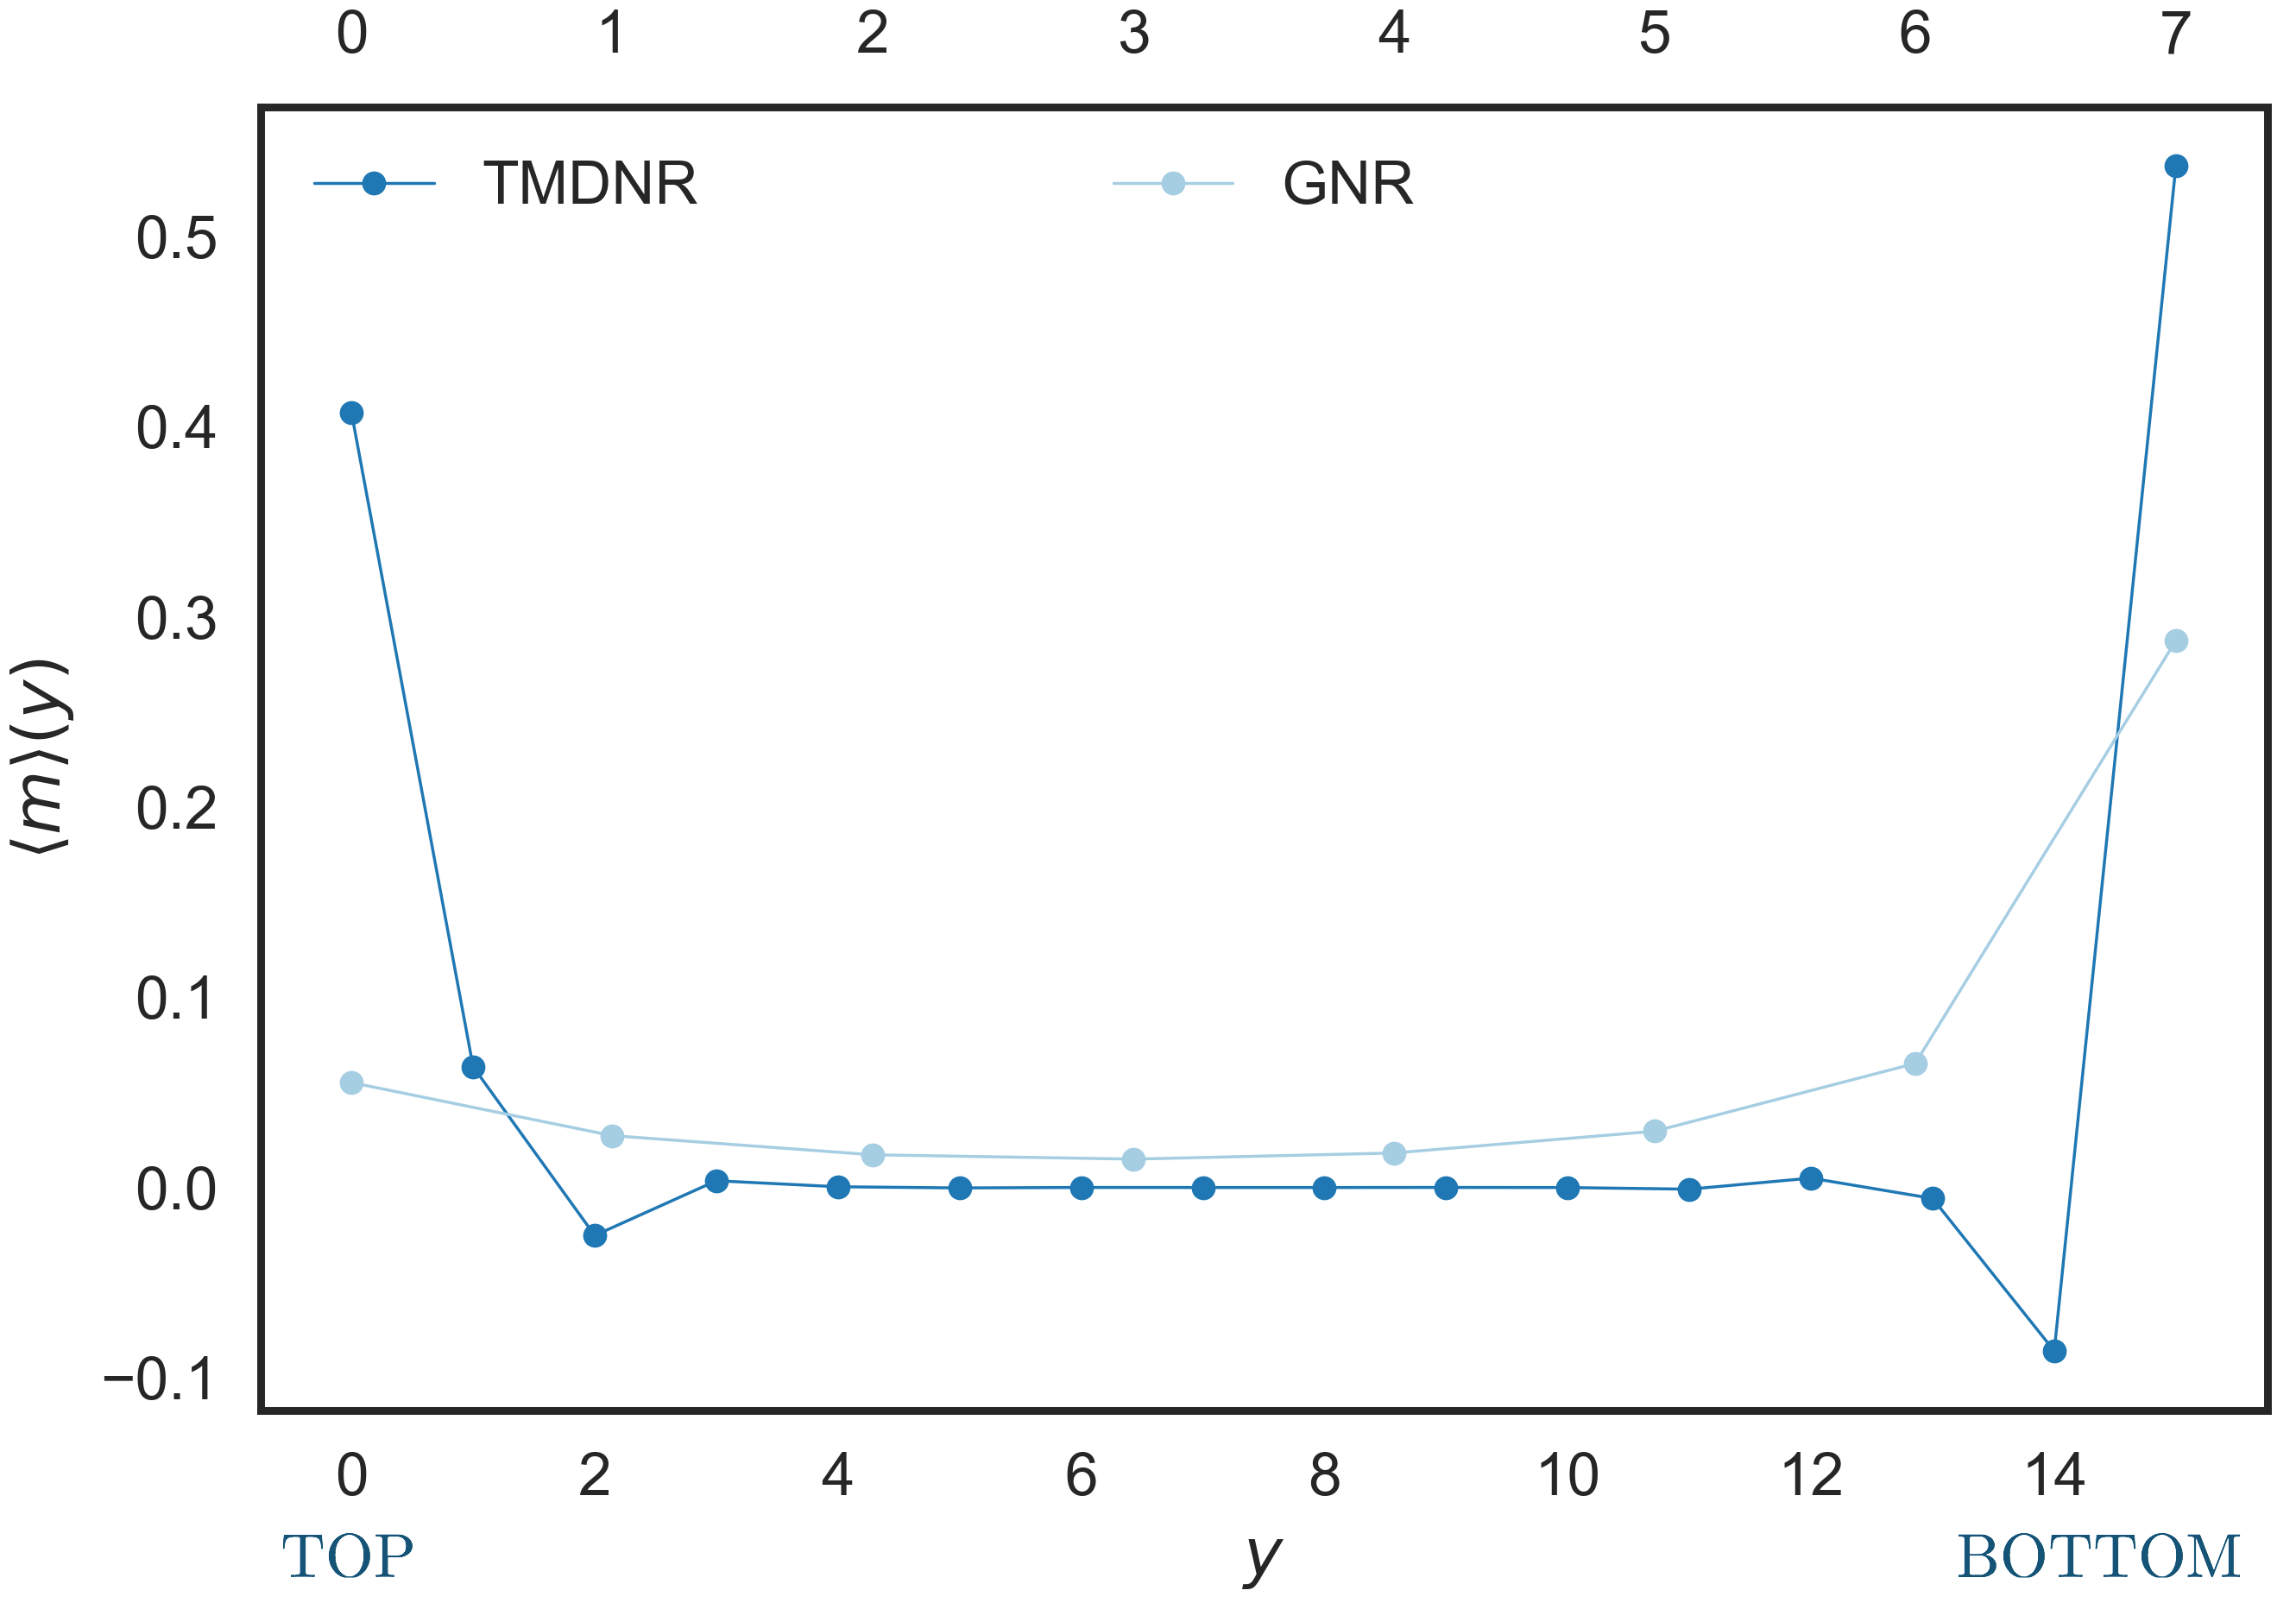
\includegraphics[scale=0.462]{Applications/magProf.png}
	\caption[Comparison between the MF solutions of the Hubbard model for a graphene nanoribbon (GNR) and a \acs{TMDNR}. Spin density profile along the ribbon's transverse direction.]{Left: Comparison between the MF solutions of the Hubbard model at half filling for a graphene nanoribbon (GNR) at $U=1.2$ with $\beta t = 20$ (left) and a \acs{TMDNR}.
	Right: Comparison between the spin density profile along the ribbon's transverse direction $\left\langle m \right\rangle (y)$ (the obtained solution is constant along $x$) for the GNR and the \acs{TMDNR}).}
	\label{fig:nanoGraphVsTMD}
\end{figure}

